\newcommand{\mytitle}{Characterisation of scaled pointclasses in $L(\mathbb R)$}
\newcommand{\myauthor}{Dan Saattrup Nielsen}
%\input{/home/leidem/Dropbox/std_preamble.tex}
%\input{/home/leidem/Dropbox/art.tex}
\input{/Users/dn16382/Dropbox/std_preamble.tex}
\input{/Users/dn16382/Dropbox/art.tex}

\abstract{
	We present the characterisation of the scaled pointclasses in $L(\mathbb R)$ under determinacy hypotheses, given in \cite{Steel}. The proof that $\Sigma_1^{J_\alpha(\mathbb R)}$ has the scale property under $\Det(J_\alpha(\mathbb R))$ is given in full, to give an idea of how the scales are constructed, and the rest of the results are then given with references. The characterisation is summed up in Corollary \ref{coro.characterisation} and in the diagram given in the appendix.
}

\section{Constructing scales from games}

For basic definitions of scales and scaled pointclasses see e.g. \cite{Kechris}. We'll be using a game-theoretic way of producing scales, originally due to \cite{Mos} -- we need the following definition.

\defi{
	Let $P$ be a unary relation. Then $\lambda x.G_x:\mathbb R\to V$ is a \textbf{closed game representation of $P$} if there's an ordinal $\alpha$ such that every $G_x$ is a closed game on $\omega^{<\omega}\times\alpha$ of length $\omega$, and a binary relation $Q\subset(\omega^{<\omega})^{<\omega}\times\alpha^{<\omega}$ such that player I has a winning quasi-strategy in $G_x$ iff $P(x)$ holds, and $u=\bra{\vec s,\vec\beta}$ is winning for player I iff
	\eq{
		Q(\bra{x\restr n,s_0\restr n,\hdots,s_n\restr n},\bra{\beta_0,\hdots,\beta_n})
	}

	holds, where $n=\lh(u)$.
}

For a closed game representation $\lambda x.G_x$ of $P$, say $P_k(x,u)$ holds iff $u$ is a partial play in $G_x$ of length $k$ from which player I has a winning quasi-strategy in $G_x$. Then a ``refinement'' of Theorem 1 in \cite{MS}, building on a scale construction in \cite{Mos}, showed that if $\gamma\in\on$ is such that $\alpha<\omega\gamma$ and $P_k\in J_\gamma(\mathbb R)$ for all $k<\omega$, then $\Det(J_\gamma(\mathbb R))$ implies that there's a scale on $P$ in $J_\gamma(\mathbb R)$. This is the strategy we'll be using in the proof of the following theorem (and indeed, it's the strategy used to construct the scales appearing in all theorems cited in this note).

\pagebreak
\theo[Steel]{
	\label{theo.scale}
	If $\alpha>0$ and $\Det(J_\alpha(\mathbb R))$ then $\Sigma_1^{J_\alpha(\mathbb R)}$ has the scale property.
}
\proof{
The case where $\alpha$ is a successor ordinal turns out to just be a slightly more technical version of the limit case, so we deal with the limit case first.

\qquad Let $\varphi_0(v)$ be $\Sigma_1$ and say $P(x)$ holds iff $J_\alpha(\mathbb R)\models\varphi_0[x]$ for $x\in\mathbb R$, and furthermore for $\beta<\alpha$ say $P^\beta(x)$ holds iff $J_\beta(\mathbb R)\models\varphi_0[x]$. The plan is then to construct closed game representations for every $P^\beta$ and then ``glue'' the corresponding scales together to get a scale $\bra{\psi_n\mid n<\omega}$ on $P$. We want to make sure that $\vec\psi$ is a $\Sigma_1^{J_\alpha(\mathbb R)}$-scale though, which we'll see is the case from the fact that the prewellorderings associated to the ``approximating'' scales are all elements of $J_\alpha(\mathbb R)$.

\qquad Let's then describe the game $G_x^\beta$ associated to $P^\beta$. A typical run is as follows.
\game{i_0,x_0,\eta_0}{x_1}{i_1,x_2,\eta_1}{x_3}{\dots}{\dots}{}{}

where $i_k\in\{0,1\}$, $x_k\in\mathbb R$ and $\eta_k<\omega\beta$. Now, to be able to describe the winning conditions of the game, we first need to describe a certain theory $T$. The theory will be in the extended language $\mathcal L:=\mathcal L_\in\cup\{\dot x_i\mid i<\omega\}$. First fix recursive injective maps $m,n:\form(\mathcal L)\to\{2n\mid n\in[1,\omega)\}$ with disjoint ranges. Then $T$ consists of the following sentences:
\begin{enumerate}
	\item[$(1)\phantom{_\varphi}$] Extensionality;
	\item[$(2)\phantom{_\varphi}$] $V=L(\mathbb R)$;
	\item[$(3)_\varphi$] $\exists v\varphi(v)\to\exists v(\varphi(v)\land\forall u\in v\lnot\varphi(u))$;
	\item[$(4)_{i\ }$] $\dot x_i\in\mathbb R$;
	\item[$(5)\phantom{_\varphi}$] $\varphi_0(\dot x_0)\land\forall\delta(J_\delta(\mathbb R)\not\models\varphi[\dot x_0])$;
	\item[$(6)_\varphi$] $\exists v\varphi(v)\to\exists v\exists F(\varphi(v)\land\vartheta_0(F,\dot x_{m(\varphi)},v))$;
	\item[$(7)_\varphi$] $\exists v(\varphi(v)\land v\in\mathbb R)\to\varphi(\dot x_{n(\varphi)})$.\\
\end{enumerate}

In $(6)$, $\vartheta_0$ describes the graph of the uniformly definable surjection $f_\gamma:[\omega\gamma]^{<\omega}\times\mathbb R\to J_\gamma(\mathbb R)$ for all $\gamma$. $\vartheta_0$ can be chosen to be $\Sigma_1$.

\qquad Now, let's return to our definition of $G_x^\beta$. For a partial play $u:=\bra{\bra{i_k,x_{2k},\eta_k,x_{2k+1}},\mid k<n}$ of $G_x^\beta$, $T^*(u):=\bigcup\{\vartheta\mid\vartheta\text{ is an $\mathcal L$-sentence}\land i_{n(\vartheta)}=0\}$ and $T^*(p):=\bigcup\{T^*(p\restr n)\mid n<\omega\}$ for a play $p$. We then define such a play to be winning for player I iff
\begin{enumerate}
	\item[(a)] $x_0=x$;
	\item[(b)] $T^*(p)$ is a complete and consistent extension of $T$ such that $\godel{\dot x_i(n)=m}\in T^*(p)$ iff $x_i(n)=m$, for all $i,m,n$;
	\item[(c)] For $\varphi(v),\psi(v)\in\Form(\mathcal L)$ and assuming that $\godel{\iota v\varphi(v)\in\on\land\iota v\psi(v)\in\on}\in T^*(p)$ then $\godel{\iota v\varphi(v)\leq\iota v\psi(v)}\in T^*(p)$ iff $\eta_{n(\varphi)}\leq\eta_{n(\psi)}$.\\
\end{enumerate}

Here $\iota v\varphi(v)$ is an abbreviation for ``the unique $v$ such that $\varphi(v)$''. This finishes the definition of $G_x^\beta$. To show that it works, we'll show that player I wins $G_x^\beta$ iff he's playing ``honestly'', in analogy with the canonical quasi-strategy of ``not losing'' for closed games. To define honesty, let again $u$ be a partial play of $G_x^\beta$ as above. Then $u$ is $(\beta,x)$-honest iff $J_\beta(\mathbb R)\models\varphi_0[x]$ and, letting $\gamma\leq\beta$ be least such that $J_\gamma(\mathbb R)\models\varphi_0[x]$, then
\begin{enumerate}
	\item[(i)] $n>0\to x_0=x$; and
	\item[(ii)] Letting $\dot x_i^{J_\gamma(\mathbb R)}=x_i$ for $i<2n$, then $J_\gamma(\mathbb R)\models T^*(u)\cup T$; and
	\item[(iii)] Letting $\vartheta_0,\dots,\vartheta_m$ be all $\mathcal L$-formulae $\vartheta(v)$ such that $n(\vartheta)<n$ and $J_\gamma(\mathbb R)\models\iota v\vartheta(v)\in\on$, and letting $\delta_i<\omega\gamma$ be such that $J_\gamma(\mathbb R)\models\iota v\vartheta_i(v)=\delta$, then $\delta_i\mapsto\eta_{n(\vartheta_i)}$ is well-defined and extendible to an order-preserving map of $\omega\gamma$ into $\omega\beta$.
\end{enumerate}

This finishes all our definitions. The ``meat'' of the argument is then the following claim, showing that we've chosen the correct combination of games and honesty.

\clai{
	Let $u$ be a partial play of $G_x^\beta$. Then player I has a winning quasi-strategy in $G_x^\beta$, starting from $u$, iff $u$ is $(\beta,x)$-honest.
}

\cproof{
	$(\Rightarrow)$ Let $u$ be a $(\beta,x)$-honest partial play of length $n$. Then it's simple to check that player I can play some $\bra{i,y,\eta}$ such that no matter what real $z$ player II plays, $u^{\frown}\bra{i,y,\eta,z}$ is still $(\beta,x)$-honest. Also, no honest partial play is losing for player I, so playing honestly from $u$ is a winning quasi-strategy for player I. For $(\Leftarrow)$, let $\vartheta$ be the entire sentence we want to prove, i.e.
	\eq{
		\vartheta:=\ulcorner&\text{For all $\beta,x,u$, if player I has a winning quasi-strategy}\\
		&\text{starting from $u$ then $u$ is $(\beta,x)$-honest}\urcorner.
	}

	It suffices to show that $M\models\vartheta$ whenever $M$ is a countable and transitive structure satisfying a sufficiently large fragment of $\zf+\dc$ -- so let $M$ be such a model and assume that
	\eq{
		\M\models\godel{\Sigma\text{ is a winning quasi-strategy for player I in $G_x^\beta$, starting from $u$}}.
	}

	In $M$, define the poset
	\eq{
		\mathbb P:=\{v\mid v\text{ is a partial play in $G_x^\beta$ extending $u$ and following $\Sigma$}\}	
	}

	with reverse inclusion. Let $g\subset\mathbb P$ be $M$-generic and $p:=\bigcup g$, which can be seen as a ``generic run'' of $G_x^\beta$ following $\Sigma$. Further, $p$ satisfies the requirements for being a winning play for player I, as these requirements are closed. Thus $T^*(p)$ is a complete and consistent extension of $T$, so fix $\M\models T^*(p)$ and define a substructure $\N\subset\M$ as
	\eq{
		\N:=\{b\in\M\mid\exists i<\omega\exists\psi(&\psi\in\form(\mathcal L)\land\psi\text{ has no constant symbols}\\
			&\text{but $\dot x_i$ and }b=\iota v(\M\models\psi[v])\}.
	}

	By axioms $(3)$ and $(6)$ of $T$ we get that $\N\prec\M$. Write
	\eq{
		p=\bra{\bra{i_k,x_{2k},\eta_k,x_{2k+1}}\mid k<\omega}.
	}
	
	Whenever $b\in o(\N)$ and $b=\iota v(\M\models\psi[v])$ then let $f(b):=\eta_{n(\psi)}$. Requirement $(c)$ of $G_x^\beta$ shows that $f:o(\N)\to\omega\beta$ is well-defined and order-preserving, so $N$ is wellfounded and we may then assume that $\N=J_\gamma(\mathbb R^{\M})$ with $\dot x_i^{\N}=x_i$ (from $p$).

	\qquad By axiom $(5)$ of $T$ and $(a)$ of $G_x^\beta$, $\gamma$ is least such that $J_\gamma(\mathbb R)\models\varphi_0[x]$. Then conditions $(i)-(iii)$ of honesty are easy to check, with the map $f$ being the witness for $(iii)$. By absoluteness of honesty we get that $u$ is $(\beta,x)$-honest in$ \M$ as well, proving the claim.
}

Note that the claim then implies that player I has a winning quasi-strategy in $G_x^\beta$ iff $J_\beta(\mathbb R)\models\varphi_0[x]$. Letting $P_n^\beta(x,u)$ iff player I has a winning quasi-strategy in $G_x^\beta$ from the length $n$ partial play $u$, we see that this holds iff $u$ has length $n$ and is $(\beta,x)$-honest, so that $P_n^\beta\in J_{\beta+1}(\mathbb R)$ for every $\beta$ and $n$, and also that the map $(\beta,n)\mapsto P_n^\beta$ is $\Sigma_1^{J_\alpha(\mathbb R)}$. This shows that there is a $\Sigma_1^{J_\alpha(\mathbb R)}$-scale on $P^\beta$.

\qquad We can then define a scale $\vec\psi$ on $P$ as $\psi_0(x):=\mu\beta P^\beta(x)$ and recursively setting $\psi_{k+1}(x):=\bra{\psi_0(x),\varphi_k^{\psi_0(x)}(x)}$ with $\vec{\varphi^\beta}$ being the scale on $P^\beta$ and $\bra{\cdot,\cdot}$ being a coding of pairs of ordinals to ordinals. Then $\vec\psi$ is furthermore $\Sigma_1^{J_\alpha(\mathbb R)}$, so we're then done, as long as $\alpha$ is a limit ordinal.

\qquad For general $\alpha$ the strategy is almost the same: again let $P(x)$ iff $J_\alpha(\mathbb R)\models\varphi_0[x]$ for some $\Sigma_1$-formula $\varphi_0$. Let $\beta<\alpha$.

\clai{
	There's a first-order $\psi_n$, for each $n<\omega$, such that $J_\beta(\mathbb R)\models\psi_n[x]$ iff $S_{\omega\beta+n}(\mathbb R)\models\varphi_0[x]$.
}

\cproof{
	Recall that Jensen's $S$-function is rudimentary and so also \textit{simple}, meaning that we can substitute any free variable $x$ in a $\Sigma_0$-formula with $S(x)$ and still end up with a $\Sigma_0$-formula. We can use this property to find a $\Sigma_0$-formula $\psi$ such that for any transitive $M$ and $x\in M$,
	\eq{
		\psi(M,x)\quad\text{iff}\quad S^n(M)\models\varphi_0[x].
	}

	Given $\psi$, we can cook up a first-order $\psi_n$ such that $(M\models\psi_n[x])$ iff $\psi(M,x)$, so that replacing $M$ with $J_\beta(\mathbb R)$ we get the wanted.
}

Now for each $\beta<\alpha$ and $n<\omega$ we can define a game $G_x^{\beta,n}$ such that player I wins iff $\exists\gamma\leq\beta(J_\gamma(\mathbb R)\models\psi_n[x])$ iff $S_{\omega\beta+n}(\mathbb R)\models\varphi_0[x]$, so that by ``chopping'' the games $G_x^\beta$ into the $\omega$ many pieces $G_x^{\beta,n}$ we can effectively do the same as in the limit case. We just have to replace axiom $(5)$ of $T$ with
\eq{
	(5)^*\ \psi_n(\dot x_0)\land\forall\delta(J_\delta(\mathbb R)\models\lnot\psi_n(\dot x_0)).
}

We can then define $(\beta,n,x)$-honesty and prove the corresponding claim as before, finishing the proof of the theorem.
}

Since there's a $\Sigma_1^{J_\alpha(\mathbb R)}$ set of reals universal for $\Sigma_1^{J_\alpha(\mathbb R)}(\mathbb R)$ sets of reals, we get the following corollary.

\qcoro{
	If $\alpha>0$ and $\Det(J_\alpha(\mathbb R))$ then $\Sigma_1^{J_\alpha(\mathbb R)}(\mathbb R)$ has the scale property.
}


\section{Characterisation of scaled pointclasses of $L(\mathbb R)$}

This section will answer the question of which values of $n<\omega$ and $\alpha\in\on$ implies that $\bSigma_n^{J_\alpha(\mathbb R)}$. Theorem \ref{theo.scale} shows that this is at least the case if $n=1$ and if real parameters suffices to parametrise all of $J_\alpha(\mathbb R)$. The main tool we'll use here is the notion of a \textit{gap}.

\defi{
	Let $\alpha<\beta\in\on$. Then the closed interval $[\alpha,\beta]$ is a \textbf{gap} if $J_\alpha(\mathbb R)\prec_{\Sigma_1}^{\mathbb R} J_\beta(\mathbb R)$ and this stops being true for smaller values of $\alpha$ or larger values of $\beta$.
}

\lemm{
	The gaps partition $\Theta^{L(\mathbb R)}$.
}
\proof{
	Given any $\gamma<\Theta^{L(\mathbb R)}$ we can simply let $\alpha\leq\gamma$ be least such that $J_\alpha(\mathbb R)\prec_{\Sigma_1}^{\mathbb R} J_\gamma(\mathbb R)$ and $\beta\geq\alpha$ the supremum of all $\delta<\Theta^{L(\mathbb R)}$ such that $J_\gamma(\mathbb R)\prec_{\Sigma_1}^{\mathbb R} J_\delta(\mathbb R)$. Then clearly $[\alpha,\beta]$ is a gap and $\gamma\in[\alpha,\beta]$. Say now that two gaps $[\alpha,\beta]$ and $[\alpha',\beta']$ overlapped at some $\gamma$. This means that $J_\alpha(\mathbb R)\prec_{\Sigma_1}^{\mathbb R} J_\gamma(\mathbb R)$ and $J_\gamma(\mathbb R)\prec_{\Sigma_1}^{\mathbb R} J_{\beta'}(\mathbb R)$, but $J_\alpha(\mathbb R)\nprec_{\Sigma_1}^{\mathbb R}J_{\beta'}(\mathbb R)$. But this is impossible as we're requiring that all parameters lie in $\mathbb R\cup\{V_{\omega+1}\}$, $\contr$.
}

We can then split up the values of $\alpha$ into three cases, whether it begins a gap, ends a gap, or lies properly within a gap. The following result shows that we don't have the consider the last case.

\qtheo[Martin]{
	Let $[\alpha,\beta]$ be a gap and assume $\Det(J_{\alpha+1}(\mathbb R))$. Then there's a $\Pi_1^{J_\alpha(\mathbb R)}$ subset of $\mathbb R\times\mathbb R$ with no $\bSigma_1^{J_\beta(\mathbb R)}$ uniformisation. In particular, if $\gamma\in(\alpha,\beta)$ and $\Det(J_\gamma(\mathbb R))$ holds, then none of the classes $\bSigma_n^{J_\gamma(\mathbb R)}$ or $\bPi_n^{J_\gamma(\mathbb R)}$ have the scale property, for any $n<\omega$.
}

Let's consider the case where $\alpha$ begins a gap. The case where $n=1$ turns out to be quite simple, given our Theorem \ref{theo.scale} above.

\coro{
	Let $\alpha>0$ begin a gap and assume $\Det(J_\alpha(\mathbb R))$. Then $\bSigma_1^{J_\alpha(\mathbb R)}$ has the scale property.
}
\proof{
	The thing to note here is that $\alpha$ beginning a gap implies that there's a partial $\Sigma_1^{J_\alpha(\mathbb R)}$ surjection $f:\mathbb R\to J_\alpha(\mathbb R)$. Indeed, by forming $\h:=\chull_1^{J_\alpha(\mathbb R)}(\mathbb R\cup\{V_{\omega+1}\})$ we see that $\h=J_\alpha(\mathbb R)$ as $\alpha$ begins a gap, so the associated $\Sigma_1^{J_\alpha(\mathbb R)}$ Skolem function is then as desired. This fact along with Theorem \ref{theo.scale} then implies the wanted.
}

For the case where $n>1$ this turns out to depend on whether $\alpha$ is \textit{admissible}. Recall that $\alpha$ is \textbf{admissible} if $J_\alpha(\mathbb R)\models\textsf{KP}$, where $\textsf{KP}$ is the (quite weak) Kripke-Platek set theory. Another equivalent characterisation is that $\alpha$ is admissible iff there is no $\Sigma_1^{J_\alpha(\mathbb R)}$ cofinal map $f:\gamma\to\omega\alpha$ for $\gamma<\omega\alpha$.\footnote{Technically admissibility is defined for the $J_\alpha$ hierarchy and not the $J_\alpha(\mathbb R)$ hierarchy -- but as we'll only work with the latter during this note, there won't be any confusion.} The key thing is then the following.

\lemm{
	Assume that $\alpha$ begins a gap and is inadmissible. Then for all $n\geq 1$,
	\eq{
		\bSigma_{n+1}^{J_\alpha(\mathbb R)}=\exists^{\mathbb R}(\bPi_n^{J_\alpha(\mathbb R)})\qquad\text{and}\qquad\bPi_{n+1}^{J_\alpha(\mathbb R)}=\forall^{\mathbb R}(\bSigma_n^{J_\alpha(\mathbb R)}).\tag*{$\dashv$}
	}
}

\qcoro{
	Assume $\alpha>0$ begins a gap, is inadmissible and $\Det(J_{\alpha+1}(\mathbb R))$ holds. Then for all $n<\omega$, both $\bSigma_{2n+1}^{J_\alpha(\mathbb R)}$ and $\bPi_{2n+2}^{J_\alpha(\mathbb R)}$ have the scale property.
}

To round off the 'begins-a-gap'-case, we have the following.

\qtheo[Martin]{
	Assume $\alpha$ begins a gap, is admissible and $\Det(J_{\alpha+1}(\mathbb R))$. Then there's a $\Pi_1^{J_\alpha(\mathbb R)}$ subset of $\mathbb R\times\mathbb R$ with no uniformisation in $J_{\alpha+1}(\mathbb R)$. In particular, none of the classes $\bSigma_n^{J_\alpha(\mathbb R)}$ or $\bPi_n^{J_\alpha(\mathbb R)}$ have the scale property, for $n>1$.
}

This finishes the situation where $\alpha$ begins a gap, so let's now consider the last case in which it ends one. For this we again need a definition.

\defi{
	A gap $[\alpha,\beta]$ is \textbf{strong} if for every $b\in J_\beta(\mathbb R)$ there is an $\gamma<\beta$ and an $a\in J_\gamma(\mathbb R)$ such that for every $\vartheta(v)\in\Sigma_1\cup\Pi_1$ it holds that
	\eq{
		J_\gamma(\mathbb R)\models\vartheta[a]\quad\text{iff}\quad J_\beta(\mathbb R)\models\vartheta[b].
	}

	Otherwise $[\alpha,\beta]$ is \textbf{weak}.
}

It turns out that for us to have any chance of finding scales at the end of gaps, we have to require our gaps to be weak.

\qtheo[Martin]{
	Let $[\alpha,\beta]$ be a strong gap and assume $\Det(J_{\alpha+1}(\mathbb R))$. Then there's a $\Pi_1^{J_\alpha(\mathbb R)}$ relation which has no uniformisation in $J_{\beta+1}(\mathbb R)$. In particular, none of the classes $\bSigma_n^{J_\beta(\mathbb R)}$ or $\bPi_n^{J_\beta(\mathbb R)}$ have the scale property, for $n<\omega$.
}

If we now \textit{do} have a weak gap, we're still not sure if we can find scales at the end of it. It might be the case that $\rho_k(J_\beta(\mathbb R))>0$ for every $k\leq n$, which would mean that we simply don't have any new subsets of reals, meaning $\bSigma_n^{J_\beta(\mathbb R)}=\bSigma_n^{J_\alpha(\mathbb R)}$ and $\bPi_n^{J_\beta(\mathbb R)}=\bPi_n^{J_\alpha(\mathbb R)}$ for all $n<\omega$, reducing the case to the begins-a-gap case. But if we require this to not be the case, scales appear.

\qtheo[Steel]{
	Let $[\alpha,\beta]$ be a weak gap and assume $\Det(J_{\alpha+1}(\mathbb R))$. If $n$ is least such that $\rho_n(J_\beta(\mathbb R))=\mathbb R$ then $\bSigma_{n+2k}^{J_\beta(\mathbb R)}$ and $\bPi_{n+2k+1}^{J_\beta(\mathbb R)}$ have the scale property for every $k<\omega$.
}

The proof of the above theorem is a technical tour de force through a variation of the above proof of Theorem \ref{theo.scale}. Summing it all up, we have the following characterisation. For the $\bSigma$-case, see also the diagram in the appendix.

\qcoro{
	\label{coro.characterisation}
	Let $\alpha\in\on$ and $n<\omega$. Then
	\begin{enumerate}
		\item $\bSigma_n^{J_\alpha(\mathbb R)}$ has the scale property iff
			\begin{enumerate}
				\item $\alpha=0$ and $n$ is even; or
				\item $\alpha>0$ begins a gap and $n=1$; or
				\item $\alpha>0$ begins a gap, is inadmissible and $n>1$ is odd; or
				\item $\alpha>0$ ends a weak gap, $n$ is even and $\rho_k(J_\alpha(\mathbb R))=\mathbb R$ for some $k\leq n$.\\
			\end{enumerate}
		\item $\bPi_n^{J_\alpha(\mathbb R)}$ has the scale property iff
			\begin{enumerate}
				\item $\alpha=0$ and $n$ is odd; or
				\item $\alpha>0$ begins a gap, is inadmissible and $n>1$ is even; or
				\item $\alpha>0$ ends a weak gap, $n$ is odd and $\rho_k(J_\alpha(\mathbb R))=\mathbb R$ for some $k<n$.
			\end{enumerate}
	\end{enumerate}
}

\bibliographystyle{apalike}
\nocite{*}
\bibliography{bib}

\pagebreak
\section*{Appendix}

\vspace*{1cm}
\hspace*{-1cm}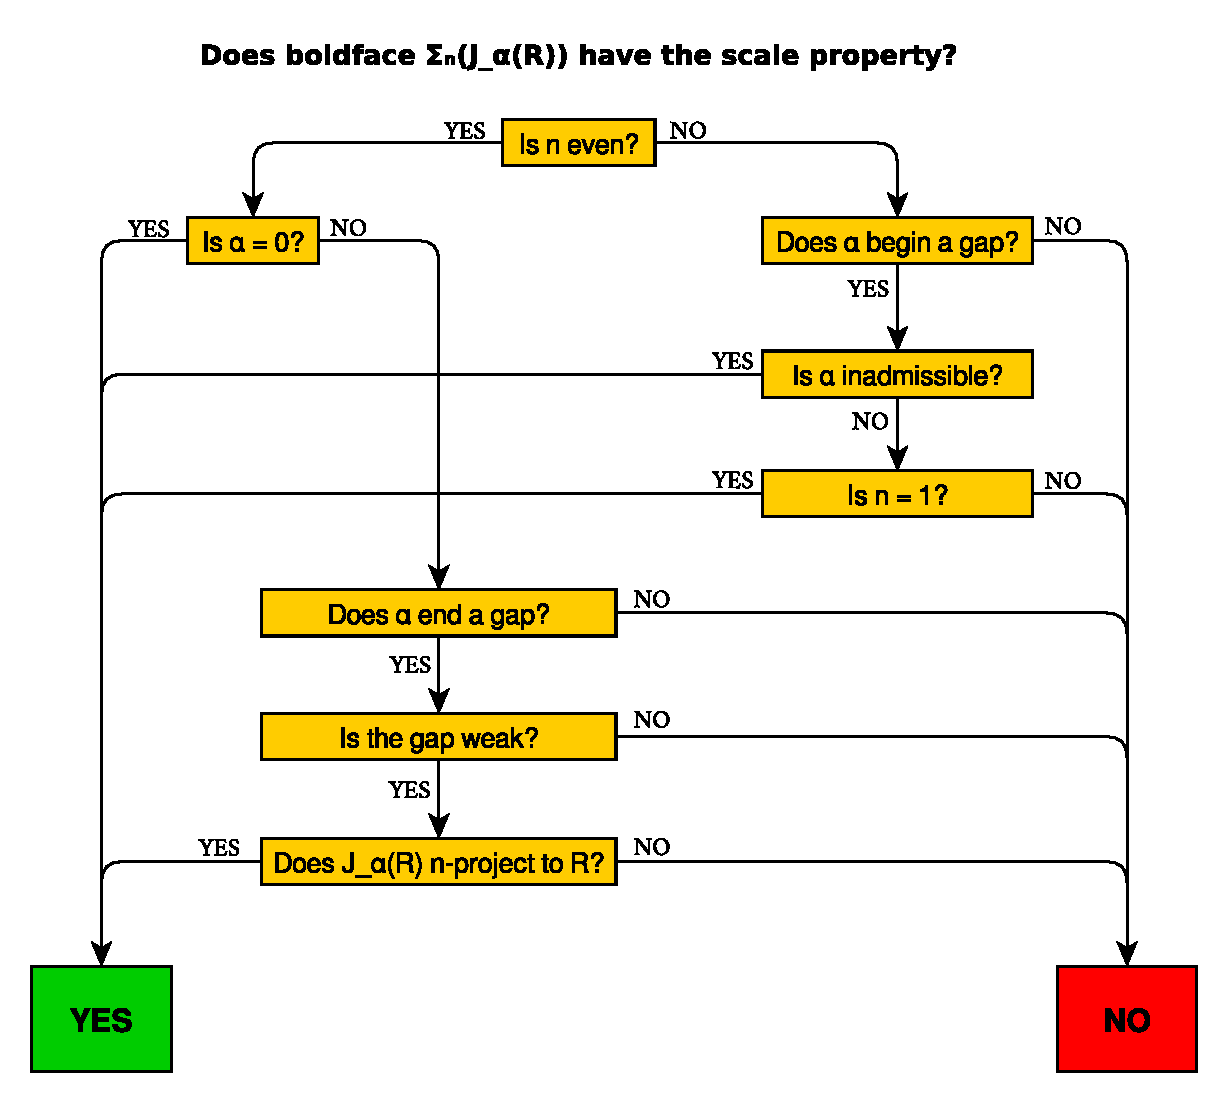
\includegraphics[scale=0.7]{gfx/scale_property.pdf}



\end{document}
